

\tikzset{every picture/.style={line width=0.75pt}} %set default line width to 0.75pt        

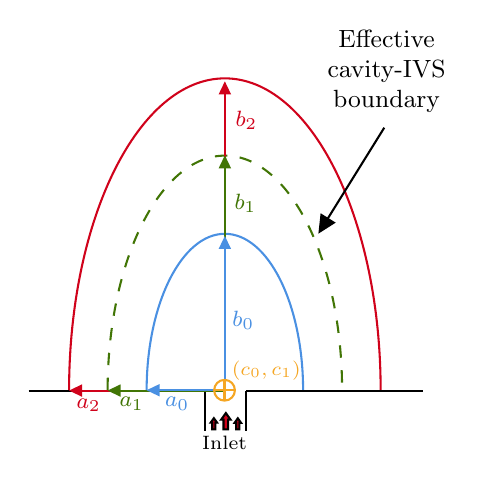
\begin{tikzpicture}[x=0.75pt,y=0.75pt,yscale=-1,xscale=1]
%uncomment if require: \path (0,300); %set diagram left start at 0, and has height of 300

%Shape: Arc [id:dp03766549009182518] 
\draw  [draw opacity=0] (43.89,241.51) .. controls (43.97,158.57) and (77.54,91.4) .. (118.94,91.4) .. controls (160.34,91.4) and (193.92,158.57) .. (194,241.51) -- (118.94,241.82) -- cycle ; \draw  [color={rgb, 255:red, 208; green, 2; blue, 27 }  ,draw opacity=1 ] (43.89,241.51) .. controls (43.97,158.57) and (77.54,91.4) .. (118.94,91.4) .. controls (160.34,91.4) and (193.92,158.57) .. (194,241.51) ;  
%Straight Lines [id:da2354434472901965] 
\draw    (109.5,241.82) -- (109.5,261.48) ;
%Straight Lines [id:da5144009246972279] 
\draw    (24.44,241.82) -- (108.75,241.82) ;
%Shape: Arc [id:dp18686074775091321] 
\draw  [draw opacity=0][dash pattern={on 4.5pt off 4.5pt}] (62.46,241.59) .. controls (62.52,179.17) and (87.79,128.62) .. (118.94,128.62) .. controls (150.1,128.62) and (175.36,179.17) .. (175.43,241.59) -- (118.94,241.82) -- cycle ; \draw  [color={rgb, 255:red, 65; green, 117; blue, 5 }  ,draw opacity=1 ][dash pattern={on 4.5pt off 4.5pt}] (62.46,241.59) .. controls (62.52,179.17) and (87.79,128.62) .. (118.94,128.62) .. controls (150.1,128.62) and (175.36,179.17) .. (175.43,241.59) ;  
%Shape: Arc [id:dp32870840671183665] 
\draw  [draw opacity=0] (81.25,241.66) .. controls (81.29,200.01) and (98.15,166.28) .. (118.94,166.28) .. controls (139.73,166.28) and (156.6,200.01) .. (156.64,241.66) -- (118.94,241.82) -- cycle ; \draw  [color={rgb, 255:red, 74; green, 144; blue, 226 }  ,draw opacity=1 ] (81.25,241.66) .. controls (81.29,200.01) and (98.15,166.28) .. (118.94,166.28) .. controls (139.73,166.28) and (156.6,200.01) .. (156.64,241.66) ;  
%Straight Lines [id:da13365761646036511] 
\draw [color={rgb, 255:red, 208; green, 2; blue, 27 }  ,draw opacity=1 ]   (118.94,241.82) -- (118.94,95.85) ;
\draw [shift={(118.94,92.85)}, rotate = 90] [fill={rgb, 255:red, 208; green, 2; blue, 27 }  ,fill opacity=1 ][line width=0.08]  [draw opacity=0] (6.25,-3) -- (0,0) -- (6.25,3) -- cycle    ;
%Straight Lines [id:da12333016540641895] 
\draw [color={rgb, 255:red, 208; green, 2; blue, 27 }  ,draw opacity=1 ]   (118.94,241.82) -- (46.89,241.82) ;
\draw [shift={(43.89,241.82)}, rotate = 360] [fill={rgb, 255:red, 208; green, 2; blue, 27 }  ,fill opacity=1 ][line width=0.08]  [draw opacity=0] (6.25,-3) -- (0,0) -- (6.25,3) -- cycle    ;
%Straight Lines [id:da33601944689998486] 
\draw [color={rgb, 255:red, 65; green, 117; blue, 5 }  ,draw opacity=1 ]   (118.94,241.82) -- (118.94,131.48) ;
\draw [shift={(118.94,128.48)}, rotate = 90] [fill={rgb, 255:red, 65; green, 117; blue, 5 }  ,fill opacity=1 ][line width=0.08]  [draw opacity=0] (6.25,-3) -- (0,0) -- (6.25,3) -- cycle    ;
%Straight Lines [id:da9639582332786008] 
\draw [color={rgb, 255:red, 65; green, 117; blue, 5 }  ,draw opacity=1 ]   (118.94,241.82) -- (65.46,241.82) ;
\draw [shift={(62.46,241.82)}, rotate = 360] [fill={rgb, 255:red, 65; green, 117; blue, 5 }  ,fill opacity=1 ][line width=0.08]  [draw opacity=0] (6.25,-3) -- (0,0) -- (6.25,3) -- cycle    ;
%Straight Lines [id:da29302727233729886] 
\draw [color={rgb, 255:red, 74; green, 144; blue, 226 }  ,draw opacity=1 ]   (118.78,241.66) -- (84.25,241.66) ;
\draw [shift={(81.25,241.66)}, rotate = 360] [fill={rgb, 255:red, 74; green, 144; blue, 226 }  ,fill opacity=1 ][line width=0.08]  [draw opacity=0] (6.25,-3) -- (0,0) -- (6.25,3) -- cycle    ;
%Straight Lines [id:da08146866090348959] 
\draw    (129.25,241.82) -- (214.25,241.82) ;
%Straight Lines [id:da2974174985117868] 
\draw    (129.25,241.82) -- (129.25,261.48) ;
%Straight Lines [id:da36914686722633006] 
\draw    (195.75,115.16) -- (165.58,163.68) ;
\draw [shift={(164,166.23)}, rotate = 301.87] [fill={rgb, 255:red, 0; green, 0; blue, 0 }  ][line width=0.08]  [draw opacity=0] (8.93,-4.29) -- (0,0) -- (8.93,4.29) -- cycle    ;
%Straight Lines [id:da06073675617036045] 
\draw [color={rgb, 255:red, 74; green, 144; blue, 226 }  ,draw opacity=1 ]   (118.94,241.82) -- (118.94,170.33) ;
\draw [shift={(118.94,167.33)}, rotate = 90] [fill={rgb, 255:red, 74; green, 144; blue, 226 }  ,fill opacity=1 ][line width=0.08]  [draw opacity=0] (6.25,-3) -- (0,0) -- (6.25,3) -- cycle    ;
%Flowchart: Or [id:dp5301694372224353] 
\draw  [color={rgb, 255:red, 245; green, 166; blue, 35 }  ,draw opacity=1 ] (113.78,241.66) .. controls (113.78,238.9) and (116.01,236.66) .. (118.78,236.66) .. controls (121.54,236.66) and (123.78,238.9) .. (123.78,241.66) .. controls (123.78,244.43) and (121.54,246.66) .. (118.78,246.66) .. controls (116.01,246.66) and (113.78,244.43) .. (113.78,241.66) -- cycle ; \draw  [color={rgb, 255:red, 245; green, 166; blue, 35 }  ,draw opacity=1 ] (113.78,241.66) -- (123.78,241.66) ; \draw  [color={rgb, 255:red, 245; green, 166; blue, 35 }  ,draw opacity=1 ] (118.78,236.66) -- (118.78,246.66) ;
%Right Arrow [id:dp5652546712623958] 
\draw  [fill={rgb, 255:red, 208; green, 2; blue, 27 }  ,fill opacity=1 ][line width=0.75]  (118.3,260.53) -- (118.3,255.8) -- (117.17,255.8) -- (119.42,252.66) -- (121.67,255.8) -- (120.54,255.8) -- (120.54,260.53) -- cycle ;
%Right Arrow [id:dp5523775393591213] 
\draw  [fill={rgb, 255:red, 208; green, 2; blue, 27 }  ,fill opacity=1 ][line width=0.75]  (112.88,260.51) -- (112.88,257.28) -- (112.11,257.28) -- (113.65,255.13) -- (115.18,257.28) -- (114.41,257.28) -- (114.41,260.51) -- cycle ;
%Right Arrow [id:dp3939210739992429] 
\draw  [fill={rgb, 255:red, 208; green, 2; blue, 27 }  ,fill opacity=1 ][line width=0.75]  (124.42,260.55) -- (124.42,257.33) -- (123.65,257.33) -- (125.18,255.18) -- (126.72,257.33) -- (125.95,257.33) -- (125.95,260.55) -- cycle ;

% Text Node
\draw (96.01,243.63) node [anchor=north] [inner sep=0.75pt]  [font=\footnotesize,color={rgb, 255:red, 74; green, 144; blue, 226 }  ,opacity=1 ]  {$a_{0}$};
% Text Node
\draw (74.01,243.63) node [anchor=north] [inner sep=0.75pt]  [font=\footnotesize,color={rgb, 255:red, 65; green, 117; blue, 5 }  ,opacity=1 ]  {$a_{1}$};
% Text Node
\draw (53.26,244.13) node [anchor=north] [inner sep=0.75pt]  [font=\footnotesize,color={rgb, 255:red, 208; green, 2; blue, 27 }  ,opacity=1 ]  {$a_{2}$};
% Text Node
\draw (121.12,207.93) node [anchor=west] [inner sep=0.75pt]  [font=\footnotesize,color={rgb, 255:red, 74; green, 144; blue, 226 }  ,opacity=1 ]  {$b_{0}$};
% Text Node
\draw (122.12,151.68) node [anchor=west] [inner sep=0.75pt]  [font=\footnotesize,color={rgb, 255:red, 65; green, 117; blue, 5 }  ,opacity=1 ]  {$b_{1}$};
% Text Node
\draw (122.62,111.43) node [anchor=west] [inner sep=0.75pt]  [font=\footnotesize,color={rgb, 255:red, 208; green, 2; blue, 27 }  ,opacity=1 ]  {$b_{2}$};
% Text Node
\draw (118.84,262.33) node [anchor=north] [inner sep=0.75pt]  [font=\Large] [align=left] {{\scriptsize Inlet}};
% Text Node
\draw (196.84,109.48) node [anchor=south] [inner sep=0.75pt]  [font=\small] [align=left] {\begin{minipage}[lt]{44.04pt}\setlength\topsep{0pt}
\begin{center}
Effective\\cavity-IVS\\boundary
\end{center}

\end{minipage}};
% Text Node
\draw (120.78,238.26) node [anchor=south west] [inner sep=0.75pt]  [font=\scriptsize,color={rgb, 255:red, 245; green, 166; blue, 35 }  ,opacity=1 ]  {$( c_{0} ,c_{1})$};


\end{tikzpicture}
